\documentclass[12pt]{article} 
\usepackage{amsmath} 
\usepackage[dvips]{graphicx}
\usepackage{multirow} 
\usepackage{multicol}
\usepackage{geometry} 
\usepackage{pdflscape}
\usepackage[labelfont=bf]{caption} 
\usepackage{setspace}
\usepackage[running]{lineno} 
% \usepackage[numbers,sort]{natbib}
\usepackage[round]{natbib} 
\usepackage{array}
\usepackage[table]{xcolor}

\newcommand{\methods}{\textit{Materials \& Methods}}
\newcommand{\SI}{\textit{Appendix}~}

\topmargin -1.5cm % 0.0cm 
\oddsidemargin 0.0cm % 0.2cm 
\textwidth 6.5in
\textheight 9.0in % 21cm
\footskip 1.0cm % 1.0cm

\usepackage{authblk}

\title{Decline of honeybees in Jumla and its consequences for crop pollination}


\author{Susanne, Alyssa, Edith, Tom, Jane, Tomas, Naomi, Sujan, Manish? (random order)} 
\date{\small$^1$Department of Agricultural Sciences\\ 
University of Helsinki\\
Helsinki, Finland
\medskip
\small$^2$ Swedish Agricultural University\\
Uppsala, Sweden\\
\medskip
$^\dagger$ Corresponding author:\\
 }

\renewcommand\Authands{ and }

\begin{document} 
\maketitle 
\raggedright
\setlength{\parindent}{15pt} 

\clearpage
\linenumbers
\begin{spacing}{2.0}https://www.overleaf.com/project/638853f7c19f734aaa6bcb3c

\section*{Abstract} 
- summary of honeybee decline based on beekeeper info and responses
- context: which honeybees are key pollinators (from applied ecology paper)
- details: which crops are honeybees (Apis cerana) most/least important for? Differences across villages? Which other insects visit the crops which are highly honeybee-dependent? does the main activity period of A. cerana overlap with highly bee-dependent crops?

\section*{Notes for the discussion}
Evidence shows that honey bees produce less honey if they need to forage at greater distances~\citep{Ribbands1951}. Solitary bees experience a reduction in reproductive success when forced to forage farther away. The breeding rate
 of a colony partly depends upon the quantity of incoming forage~\citep{Nolan1925}. Distance to suitable wild forage plants could explain the reduction in honey production per hive experienced in Jumla. 
 Weather also determines foraging range \citep{Ribbands1951}. Jumli beekeepers were repeatedly saying that bees were caught in bad weather (heavy rainfall) conditions during flights and therefore did not return nest/hives. Increasingly unpredictable weather patterns due to climate change could worsen this situation. 

An recent study using an ABM model shows that abundance is a major driver of foraging distances with decreasing food source abundance leading to larger foraging distances (Grüter and Hayes 2022).



        \begin{figure}[hb!]
        \centering
        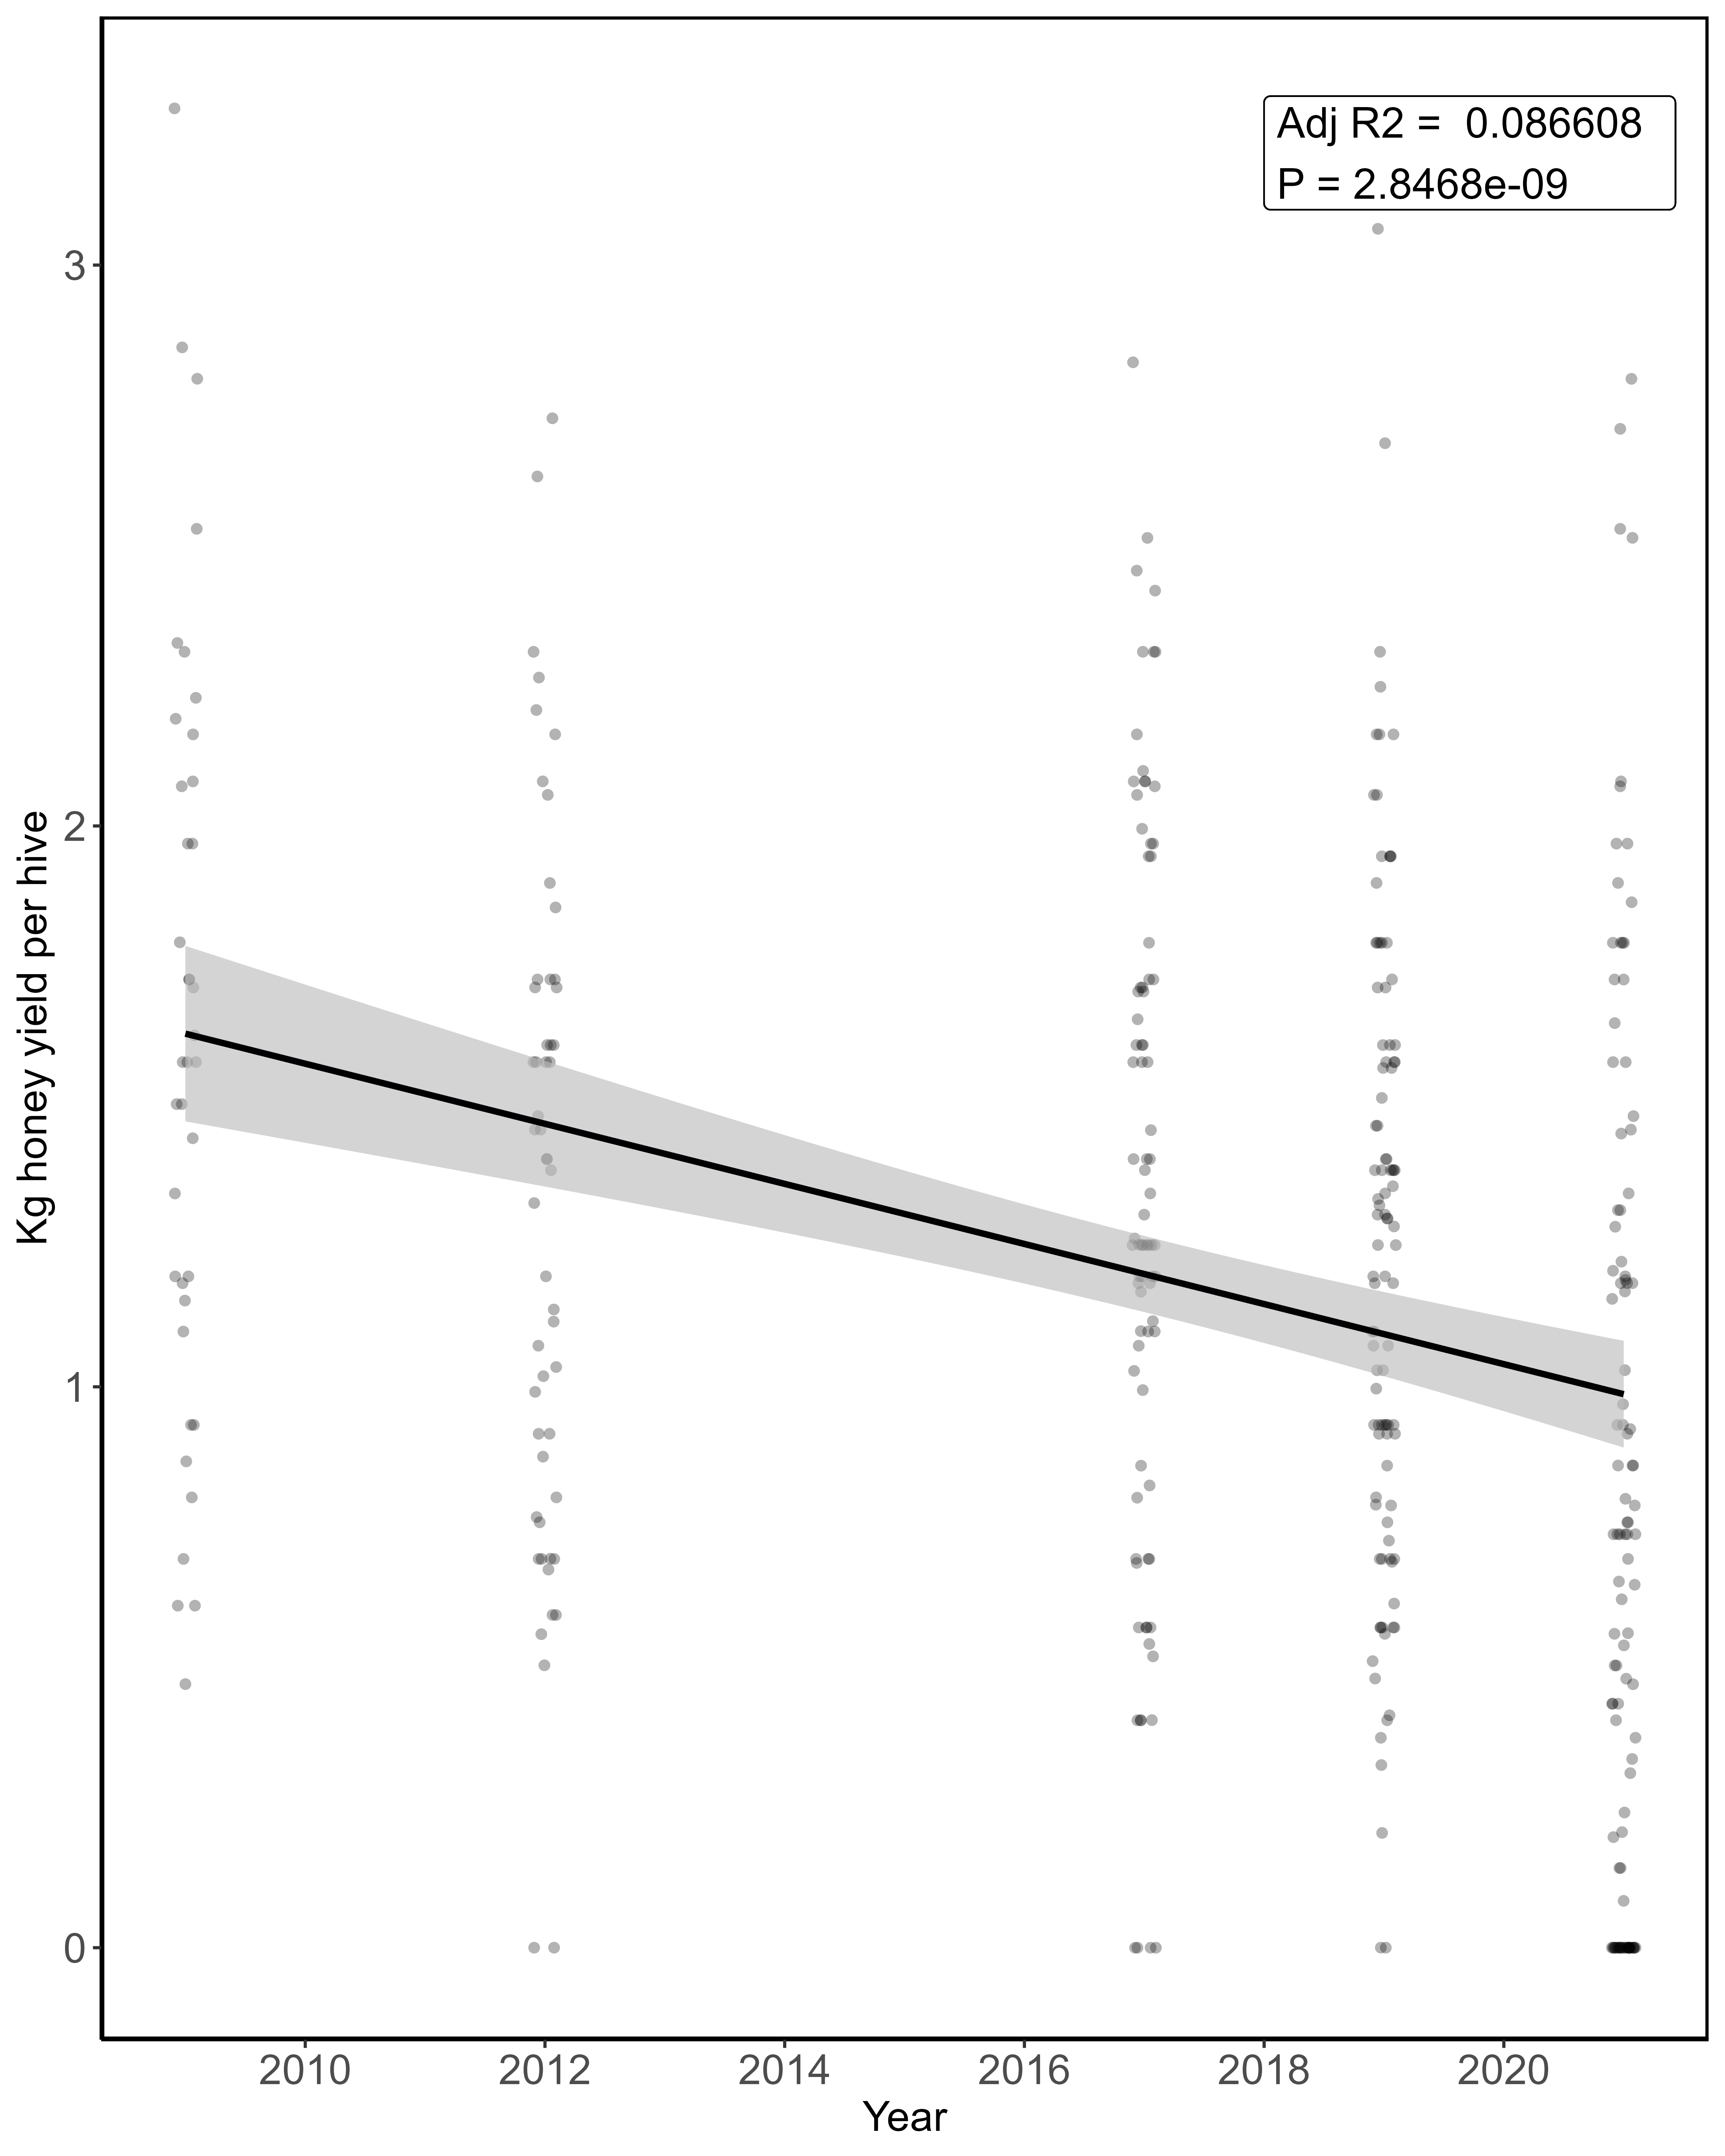
\includegraphics[height=.5\textheight]{manuscript/Figures/honey_yield_all.png}
        \caption{Change in honey yield across all villages.}
        \label{fig:honey_yield_all}
        \end{figure} 


        \begin{figure}[hb!]
        \centering
      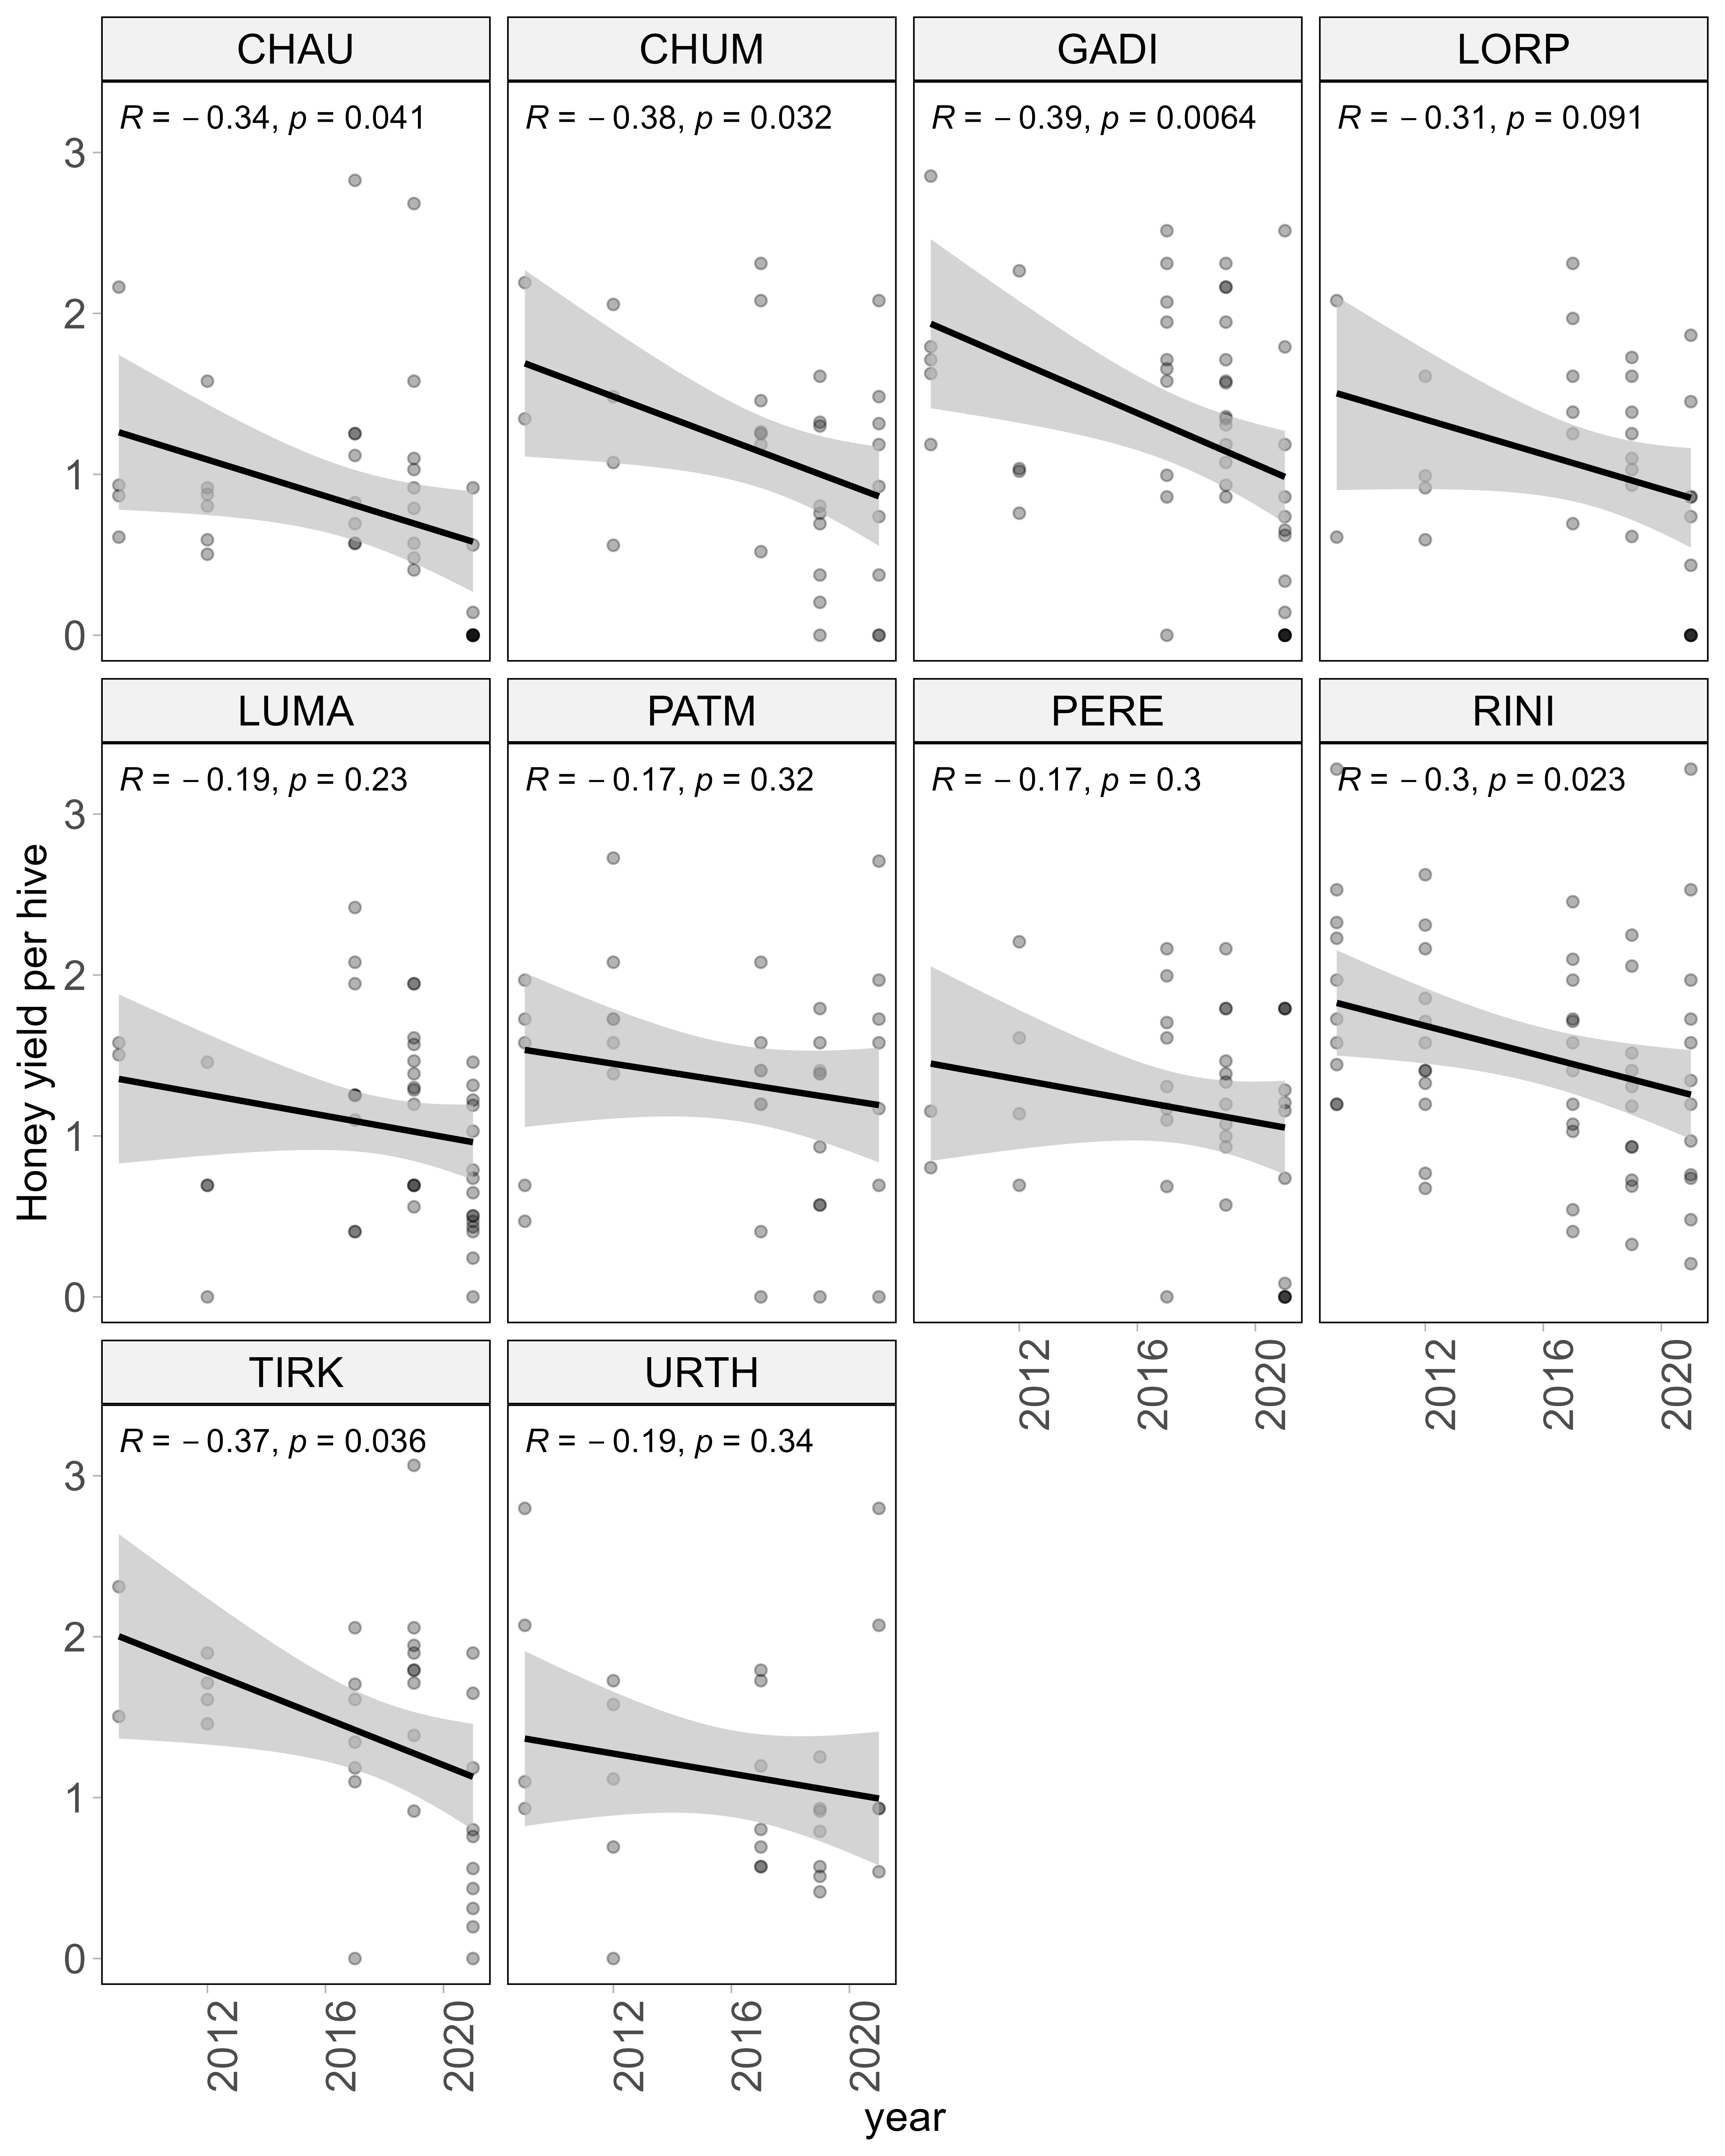
\includegraphics[height=.5\textheight]{manuscript/Figures/honey_yield_per_village.png}
        \caption{Change in honey yield per village.}
        \label{fig:honey_yield_village}
        \end{figure} 

        
% \section*{refs}
% Ribbands, C.R. (1951). The flight range of the honey-bee. J. Anim. Ecol. 20,
% 220–226.
% Nolan, W. J. (1925). 'The brood-rearing cycle of the honeybee.' Bull.U.S. Dep. Agric. Dep. no. 1349: I-55.

\end{spacing}

\clearpage

    \bibliographystyle{ecolett} 
    \bibliography{susanne}  

\end{document}
